\section{Disponibilidad de Información}
Las diferentes entidades del sistema educativo chileno y grupos de investigadores dedicados a la educación preparan y desarrollan diferentes fuentes de información que serán cruciales para el desarrollo de este proyecto.

Gracias a las fuentes de información mencionadas recientemente, y a la Ley de transparencia decrita en el capítulo 1, es posible tener acceso a la información recaudada.

A continuación se muestra en el Cuadro~\ref{fig:fuentesdeinfo} la descripción de las fuentes de información y en la Figura~\ref{fig:disponibilidadDatos}se muestra la disponibilidad de estos.

Al ver la Figura~\ref{fig:fuentesdeinfo} podemos destacar y mencionar que asegurando la calidad de estas fuentes de información y la creación de diferentes indicadores relevantes que indiquen deserción escolar se puede desarrollar una herramientas potente, pues se tiene información de el rendimiento, asistencia, características socio-económicas familiares de estudiantes, junto con caracterizaciones de vulnerabilidad, delitos y ambiente de las diferentes comunas, e inclusive isócronas\footnote{Una isócrona es un área geométrica en un mapa que muestra individuos con una misma característica, como por ejemplo misma manzana} de la manzana del colegio y/o estudiante.

\begin{figure}[H]
  \centering
    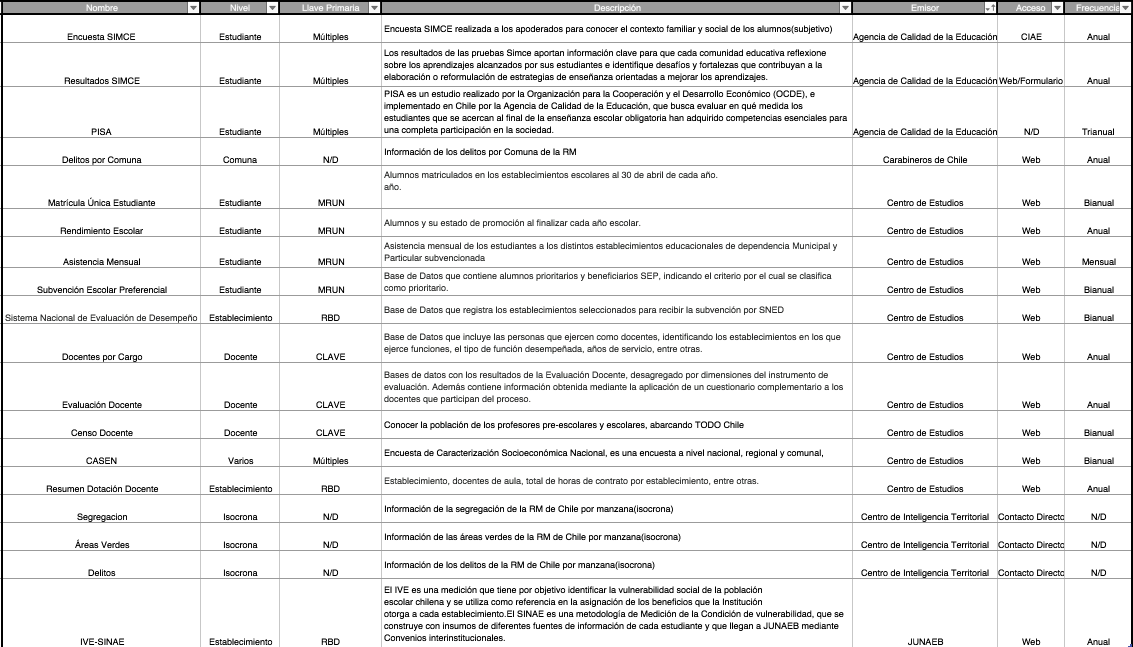
\includegraphics[width=1\textwidth,]{Figuras/fuentesdeinfo}
      \caption{Diferentes fuentes de información disponible y descripción sencilla de estas}
    \label{fig:fuentesdeinfo}
\end{figure}
\begin{figure}[H]
  \centering
    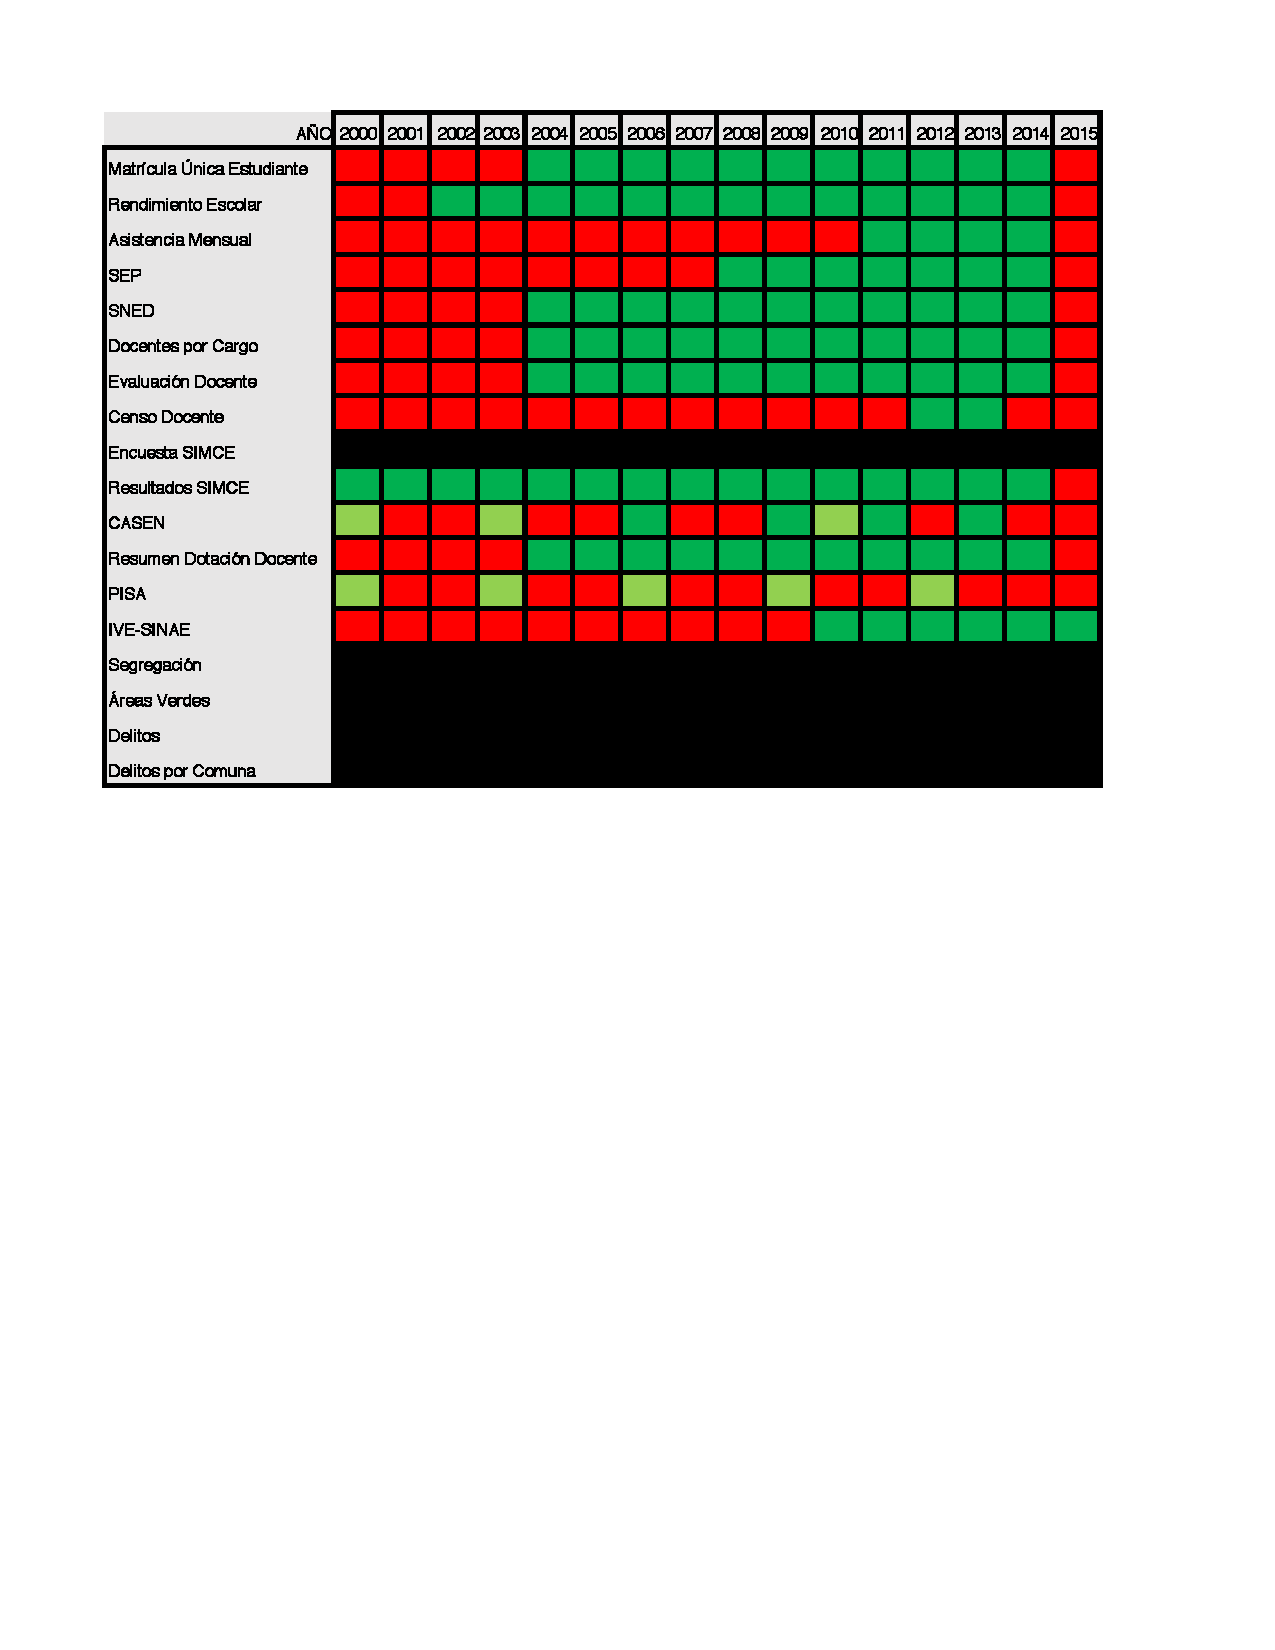
\includegraphics[trim=2cm 13cm 0cm 0cm]{Figuras/DisponibilidadDatos}
      \caption{Disponibilidad por año de las fuentes de información conocidas. El color verde indica disponibilidad y el rojo la no existencia de la fuente de información. El negro es falta de información}
    \label{fig:disponibilidadDatos}
\end{figure}
